\chapter{Photonic Reservoir Computer with Wavelength Division Multiplexed neurons}

\label{ch-wdm-rc}

In this chapter, a novel approach of \gls{prc} is proposed, in which the neurons are no longer multiplexed in time, but in wavelength (or frequency) instead. This scheme was introduced in \cite{AkroutAkram2016Pprc} and its end goal is to overcome the speed limitations imposed by the \gls{tdm} of the neurons, as exposed in section \ref{tdm-neurons-principle}. Indeed, by multiplexing the neurons in the frequency domain, the input signal can reach them all in the same time, there is no need to slow down its pace to let it alter the neurons sequentially. As an illustration, in \cite{Vandoorne2014}, they proposed the first \gls{prc} with parallelisation of the neurons. In the experiment described in the paper, the neurons were spatially multiplexed. Doing so, the authors were able to reach data processing rates up to 12.5 GHz on tasks such as header recognition or boolean logic, which is an increase of one order of magnitude compared to those reported in \cite{Vinckier2015}. This is encouraging for research in parallel \gls{prc} and motivates the study of the scheme explored in this thesis.\\

First, in section \ref{sec-scheme-wdm}, a description of the working principle is given. It starts with a high-level overview of the scheme in which different features and components are presented. After that, attention is brought to the frequency coupling mechanism used to let the neurons interact between one another. It is shown that this can be achieved using a optoelectronic \gls{pm}, even though this device has some practical drawbacks. Finally, the scheme is described with more details. In section \ref{sec-challenges-wdm}, the stabilisation issue, which is main topic of this thesis, is introduced.

%%%%%%%%%% DESCRIPTION OF THE SCHEME %%%%%%%%%%

\section{Description of the scheme}

\label{sec-scheme-wdm}

In this section, the working principle of \gls{wdm} \gls{prc} is first given. This scheme takes advantage of the wave character of light and uses different wavelength to encode the neurons. It is fibre-based and relies on an optical cavity made of a fibre loop. Inside the resonator, the different neurons need to be able to interact, therefore one has to provide some coupling mechanism for the different frequencies. This issue is tackled in section \ref{subsec-freq-coupling} and provides interesting mathematical insights that are eventually used to derive a suitable model for this other kind of linear \rcer.

%%% WORKING PRINCIPLE %%%

\subsection{Working principle}

The working principle of the new reservoir is schematised on Figure \ref{wdm_rc_principle}. The whole setup is fibre-based, and the fibre used is a polarisation maintaining, single mode fibre. 

\paragraph{Input}

The input time series $u(n)$ is converted into a continuous signal $\tilde{u}(t)$ by keeping its value constant during one period $\tau$ (sample and hold procedure), which leads to $\tilde{u}(t)=u(n)$, with $t \in [n\tau, (n+1)\tau[$. The continuous, coherent light emitted by a narrow band laser at frequency $\omega_0$ is modulated in intensity by the input signal $\tilde{u}(t)$ using a \gls{mzm}.  

\paragraph{Cavity}

The modulated data is then coupled to an optical cavity around 20 metres long\footnote{The length of the cavity can be derived from its \gls{fsr}, which is studied in the next chapter}. Inside this cavity, a \gls{pm} mixes the different optical frequencies. It is driven by a RF signal at frequency $\Omega$. More information about the \gls{pm} can be found in section \ref{subsec-freq-coupling}. Losses are introduced inside the cavity by two main sources, the intrinsic losses of the fibre and the insertion losses of the \gls{pm}, hence the presence of an intra-cavity amplifier used to compensate for them. The neurons are encoded in the electric field evolving inside this cavity, which is schematised on the figure by the three different colours for the fibre loops. Therefore, from now on, the cavity is referred to as the \textit{reservoir}. The holding time $\tau$ introduced earlier should be equal to the \gls{rtt} of the reservoir. This is done in order to update the discrete dynamics of the \rcer each time the light completes a trip around the cavity. Doing so, one ensures that the value of the neuron $x_j$ at discrete time $n+1$ depends on the values of the neurons $x_i$, with $i \in \{1,\dots, N\}$, at precisely time $n$. 

\paragraph{Readout}

The electric field encoding the neurons exits the cavity through another coupler, and is then demultiplexed in frequency. Each of the frequency component is measured using a \gls{pd}, which gives a value proportional to the squared modulus of the electric field, as explained in the previous chapter. The resulting signals are linearly combined using the trained output weights to produce the output of the reservoir $y(n)$.

\begin{equation}
	y(n) = \sum_{i=1}^{N} W_i^{\text{out}} |x_i(n)|^2
\end{equation}

\begin{figure}[h]
	\centering
	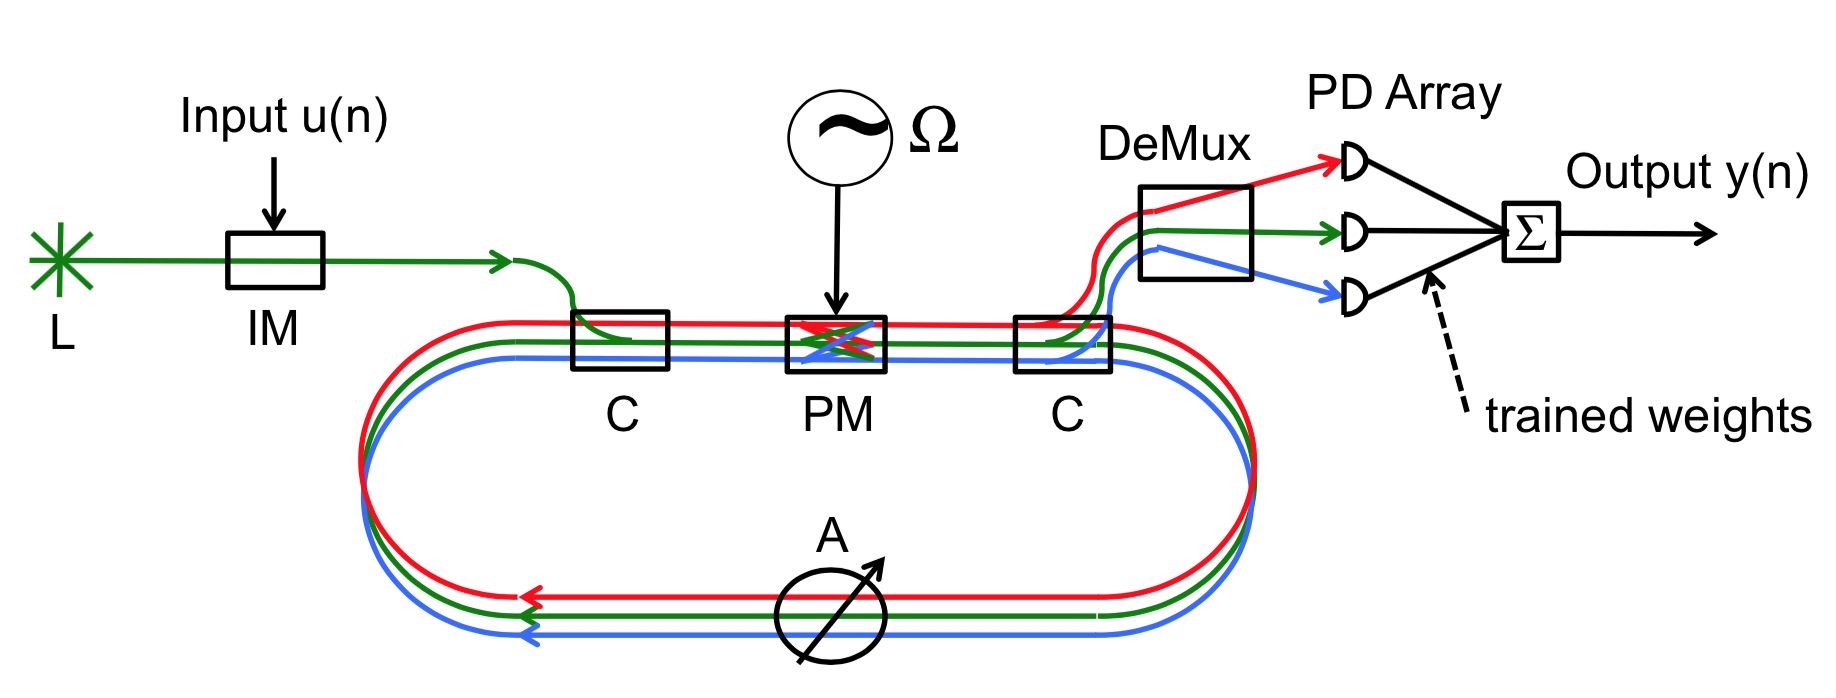
\includegraphics[width=\textwidth]{wdm_rc_principle}
	\caption{Schematic representation of the working principle of the \gls{wdm} \gls{prc} \cite{AkroutAkram2016Pprc}}
	\label{wdm_rc_principle}
\end{figure}

\paragraph{Training and testing}

The training scheme used for this setup is the batch learning. Thus, to compute the output weights $\mathbf{W}^{\text{out}}$, one can use the ridge regression technique introduced in section \ref{subsec-rc-training}. To do so, one needs to discard the first state vectors $\mathbf{x}$ because they correspond to the transient of the reservoir, and then to store them\footnote{Since the output $y$ is constructed using the squared modulus of the activation of the neurons, the matrix $\mathbf{X}$ is filled with $|x_i(n)|^2$ instead of what is said in section \ref{subsec-rc-training}, namely $x_i(n)$} as well as the desired outputs $\hat{y}$ during the whole learning period to create the matrices $\mathbf{X}$ and $\hat{\mathbf{Y}}$. After that, it is straightforward to solve equation \eqref{ridge-regression} and to find the output weights. Once the \rcer is trained, it can move on to the testing phase, during which the outputs $y(n)$ are compared to the desired outputs. From that, one can quantify the performance of the \rcer using the appropriate metric, such as the \gls{nmse} for example.

%%% FREQUENCY COUPLING OF THE NEURONS %%%

\subsection{Frequency coupling of the neurons}

\label{subsec-freq-coupling}



\begin{equation}
	Ee^{i\omega t} \underset{\Omega}{\longrightarrow} Ee^{i\omega t}e^{im\sin{(\Omega t)}} = E \sum_{n=-\infty}^{\infty} J_n(m) e^{i(\omega+n\Omega)t}
\end{equation}

\begin{figure}[h]
	\centering
	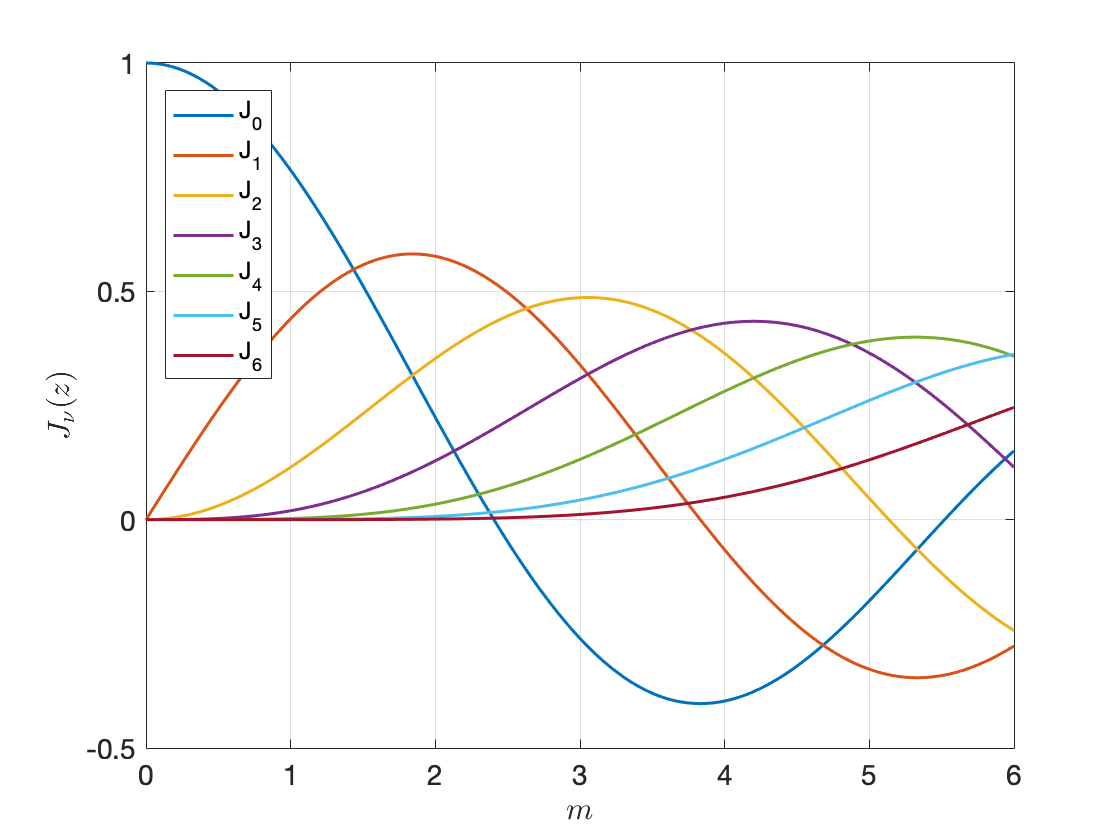
\includegraphics[width=.7\textwidth]{bessel}
\end{figure}

\begin{figure}[h]
	\centering
	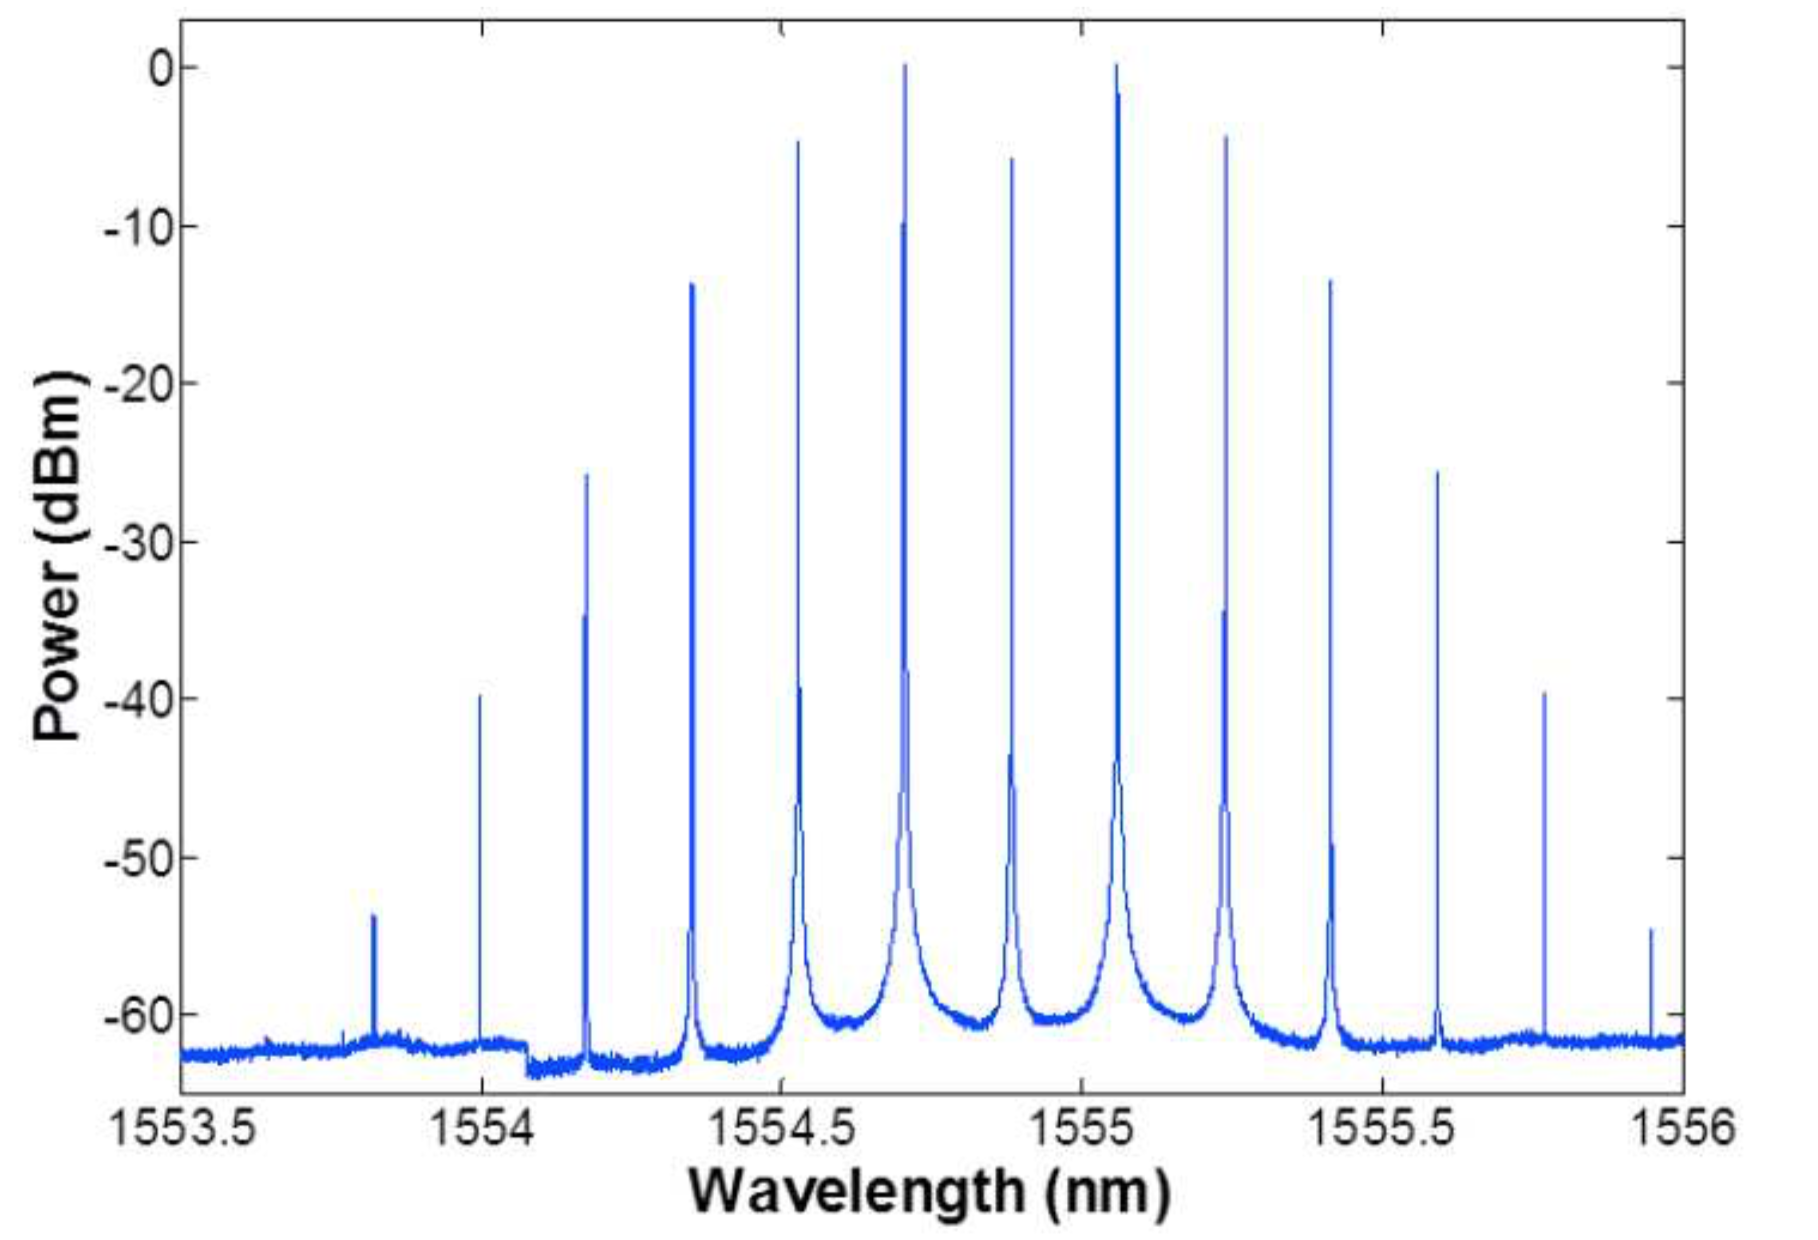
\includegraphics[width=.7\textwidth]{power-in-neurons}
	\caption{\cite{AkroutAkram2016Pprc}}
\end{figure}

%%% MATHEMATICAL MODEL %%%

\subsection{Mathematical model}

%%%%%%%%%% CHALLENGES %%%%%%%%%%

\section{Challenges}

\label{sec-challenges-wdm}

% Stabilisation
% Stabilisation signal is the same as data signal











